\documentclass{beamer}


\newcommand{\lesson}{Object-Oriented Programming, Part 3 of 3}
\newcommand{\shorttitle}{OOP3}

\author[Chris Simpkins] 
{Christopher Simpkins \\\texttt{chris.simpkins@gatech.edu}}
\institute[Georgia Tech] % (optional, but mostly needed)

\date[CS 1331]{}


\newcommand{\course}{Introduction to Object-Oriented Programming}
\subject{\course}
\title[\lesson]{\course}
\subtitle{\lesson}

\author[CS 1331]
{Christopher Simpkins \\\texttt{chris.simpkins@gatech.edu}}
\institute[Georgia Tech]

\date[]{}

\newcommand{\link}[2]{\href{#1}{\textcolor{blue}{\underline{#2}}}}
\newcommand{\code}{http://www.cs1331.org/code}

\usepackage{colortbl}

% If you have a file called "university-logo-filename.xxx", where xxx
% is a graphic format that can be processed by latex or pdflatex,
% resp., then you can add a logo as follows:

% \pgfdeclareimage[width=0.6in]{coc-logo}{cc_2012_logo}
% \logo{\pgfuseimage{coc-logo}}

\mode<presentation>
{
  \usetheme{Berlin}
  \useoutertheme{infolines}

  % or ...

 \setbeamercovered{transparent}
  % or whatever (possibly just delete it)
}

\usepackage{tikz}
% Optional PGF libraries
\usepackage{pgflibraryarrows}
\usepackage{pgflibrarysnakes}
\usepackage{pgfplots}
\usepackage{fancybox}
\usepackage{listings}
\usepackage{hyperref}
\hypersetup{colorlinks=true,urlcolor=blue}
\usepackage[english]{babel}
% or whatever

\usepackage[latin1]{inputenc}
% or whatever

\usepackage{times}
\usepackage[T1]{fontenc}
% Or whatever. Note that the encoding and the font should match. If T1
% does not look nice, try deleting the line with the fontenc.


\usepackage{listings}

% "define" Scala
\lstdefinelanguage{scala}{
  morekeywords={abstract,case,catch,class,def,%
    do,else,extends,false,final,finally,%
    for,if,implicit,import,match,mixin,%
    new,null,object,override,package,%
    private,protected,requires,return,sealed,%
    super,this,throw,trait,true,try,%
    type,val,var,while,with,yield},
  otherkeywords={=>,<-,<\%,<:,>:,\#,@},
  sensitive=true,
  morecomment=[l]{//},
  morecomment=[n]{/*}{*/},
  morestring=[b]",
  morestring=[b]',
  morestring=[b]""",
}

\usepackage{color}
\definecolor{dkgreen}{rgb}{0,0.6,0}
\definecolor{gray}{rgb}{0.5,0.5,0.5}
\definecolor{mauve}{rgb}{0.58,0,0.82}

% Default settings for code listings
\lstset{frame=tb,
  language=scala,
  aboveskip=2mm,
  belowskip=2mm,
  showstringspaces=false,
  columns=flexible,
  basicstyle={\scriptsize\ttfamily},
  numbers=none,
  numberstyle=\tiny\color{gray},
  keywordstyle=\color{blue},
  commentstyle=\color{dkgreen},
  stringstyle=\color{mauve},
  frame=single,
  breaklines=true,
  breakatwhitespace=true,
  keepspaces=true
  %tabsize=3
}


% If you wish to uncover everything in a step-wise fashion, uncomment
% the following command: 

% \beamerdefaultoverlayspecification{<+->}


\begin{document}

\begin{frame}
  \titlepage
\end{frame}

%% %------------------------------------------------------------------------
%% \begin{frame}[fragile]{SummerIntern}


%% Let's add a summer intern class to our Employee hierarchy.
%% \begin{lstlisting}[language=Java]
%% public class SummerIntern5 extends HourlyEmployee5 {

%%     public SummerIntern5(String name, Date hireDate) {
%%         this(name, hireDate, 20.00, 160.0);
%%     }
%%     public SummerIntern5(String name, Date hireDate, 
%%                         double hourlyWage, double monthlyHours) {
%%         super(name, hireDate, hourlyWage, monthlyHours);
%%     }
%%     public double monthlyPay() {
%%         Calendar rightNow = Calendar.getInstance();
%%         return isSummer(rightNow) ? super.monthlyPay() : 0.0;
%%     }
%%     // ...
%% }
%% \end{lstlisting}

%% Will this compile?

%% \end{frame}
%% %------------------------------------------------------------------------


%------------------------------------------------------------------------
\begin{frame}[fragile]{The {\tt Employee} Class Hierarchy}

Let's add a summer intern class to our Employee hierarchy.
\vspace{-.1in}
\begin{center}
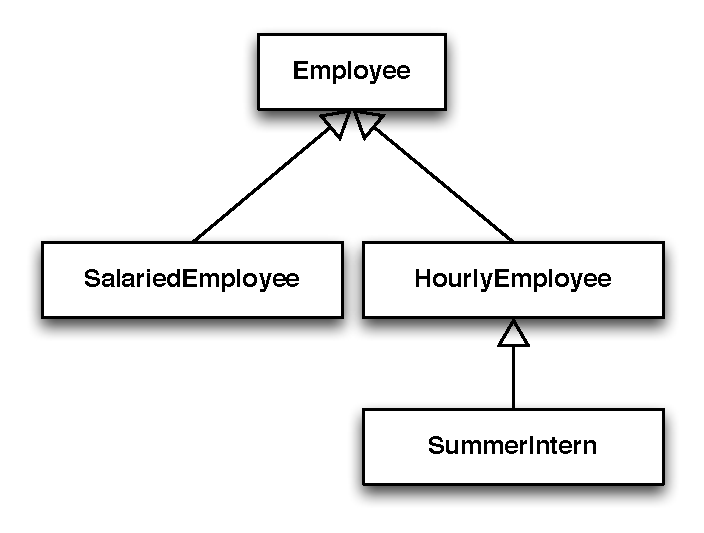
\includegraphics[height=1.5in]{expanded-employee-class-hierarchy.pdf}
\end{center}

\begin{itemize}
\item We can get the payRoll for the current month by making use of the polymorphic {\tt getMonthlyPay} method.
\item What if we wanted to get the payroll for a particular month?
\end{itemize}

Let's overload {\tt monthlyPay} so we can get the payroll for any month, not just the current month.

\end{frame}
%------------------------------------------------------------------------

%------------------------------------------------------------------------
\begin{frame}[fragile]{Enum Types}


Enums are data types that have a predefined set of constant values (\href{http://docs.oracle.com/javase/specs/jls/se7/html/jls-8.html#jls-8.9}{JLS \S 8.9}, \href{http://docs.oracle.com/javase/tutorial/java/javaOO/enum.html}{Java Enum Tutorial})

For example:
\begin{lstlisting}[language=Java]
public enum Month {
    JAN, FEB, MAR, APR, MAY, JUN, JUL, AUG, SEP, OCT, NOV, DEC
}
\end{lstlisting}
defines an enum type called {\tt Month} that can take on only one of the predefined constants {\tt Month.JAN}, {\tt Month.FEB}, ..., {\tt Month.DEC}

\begin{itemize}
\item Enum types are a class.
\item Java automatically defines convenience methods for enum types, like {\tt valueOf(String)} and {\tt values()} (See the \link{http://docs.oracle.com/javase/7/docs/api/java/lang/Enum.html}{Enum API}).
\item Because they define a class, enum types can include programmer-defined additional constructors and methods.
\end{itemize}

\end{frame}
%------------------------------------------------------------------------


%------------------------------------------------------------------------
\begin{frame}[fragile]{Overloading Methods}


An overloaded method is a set of methods with the same names but different signatures (parameter lists)\footnote{More precisely, two methods with the same name whose signatures are not {\it override-equivalent} are overloaded.} (\href{http://docs.oracle.com/javase/specs/jls/se7/html/jls-8.html#jls-8.4.9}{JLS \S 8.4.9}).\\
\vspace{.075in}
Here's an overloaded {\tt monthlyPay} for {\tt SummerIntern6}, along with a helper method demonstrating the use of the {\tt Month} enum:
\begin{lstlisting}[language=Java]
public double monthlyPay() {
    Date today = new Date();
    Month thisMonth = Month.values()[today.getMonth()];
    return monthlyPay(thisMonth);
}
public double monthlyPay(Month month) {
    return isSummer(month) ? super.monthlyPay() : 0.0;
}
private boolean isSummer(Month month) {
    return month == Month.JUN 
        || month == Month.JUL 
        || month == Month.AUG;
}
\end{lstlisting}
\vspace{-.075in}
\begin{itemize}
\item In which classes should these methods be declared? Defined?
\end{itemize}


\end{frame}
%------------------------------------------------------------------------

%------------------------------------------------------------------------
\begin{frame}[fragile]{The {\tt Employee} Class Hierarchy in UML}


\vspace{-.2in}
\begin{center}
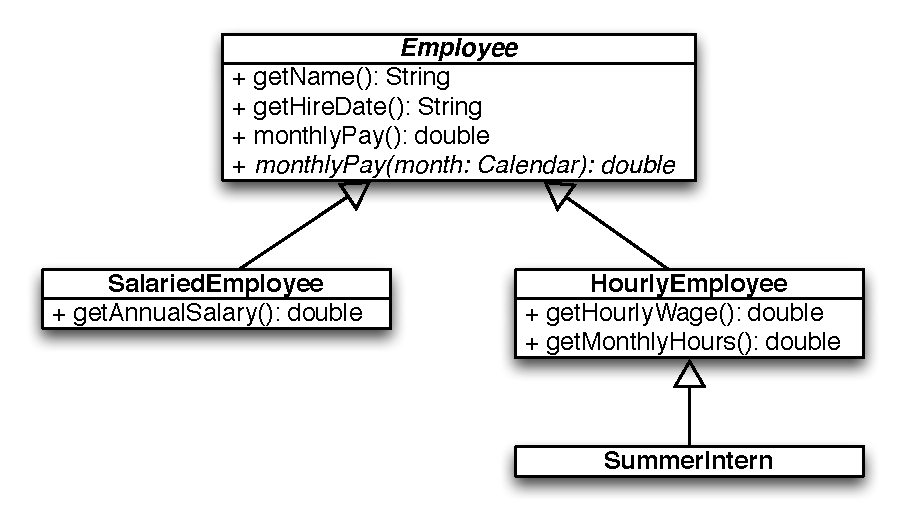
\includegraphics[height=1.5in]{employee-uml.pdf}
\end{center}
\vspace{-.25in}
\begin{itemize}
\item Italicized names are abstract (e.g., {\it Employee} is an abstract class, {\it + getMonthlyPay(month: Month)} is an abstract method).
\item We've only shown public methods (denoted by the '+' symbols in front of their names).
\item Each class has all the public methods in its superclasses, and possibly additional methods.
\item {\tt SummerIntern6} only {\it specializes} {\tt HourlyEmployee6}, that is, it modifies some behavior of its superclass but does not add any additional behavior. 
\end{itemize}


\end{frame}
%------------------------------------------------------------------------

%------------------------------------------------------------------------
\begin{frame}[fragile]{Forecasting Payroll}


Now with our overloaded  {\tt montlyPay} method we can forecast payroll:
\begin{lstlisting}[language=Java]
  Company6 c = new Company6();
  System.out.println("Monthly payroll this month: " + c.monthlyPayroll());
  System.out.printf("Monthly payroll for May: %.2f%n",
                    c.monthlyPayroll(Month.MAY));
  System.out.printf("Monthly payroll for June: %.2f%n",
                    c.monthlyPayroll(Month.JUN));
\end{lstlisting}


\end{frame}
%------------------------------------------------------------------------

%------------------------------------------------------------------------
\begin{frame}[fragile]{Inheritance Hinders Re-use}

Recall the {\tt disallowZeroesAndNegatives} method that we refactored so that it's in the {\tt Employee} class and inherited by subclasses:
\vspace{-.05in}
\begin{lstlisting}[language=Java]
public abstract class Employee6 {
    protected void disallowZeroesAndNegatives(double ... args) {
        // ...
    }
}
\end{lstlisting}

\begin{itemize}
\item There's nothing about this method that is specific to {\tt Employee}s
\item {\tt disallowZeroesAndNegatives} could be useful in other classes that are not part of the {\tt Employee} class hierarchy.
\item Since it's {\tt protected}, it can't be used outside of the {\tt Employee} class hierarchy or package. 
\end{itemize}

In software engineering terms, we say that the code in {\tt Employee} lacks {\it cohesion} - it has parts that aren't part of the {\it Employee} concept.  Such a design hinders reuse.

\end{frame}
%------------------------------------------------------------------------

%------------------------------------------------------------------------
\begin{frame}[fragile]{Favor Composition over Inheritance}

If we move these protected methods into a separate class, like \link{\code/employee/ValidationUtils.java}{ValidationUtils.java}
\begin{lstlisting}[language=Java]
public class ValidationUtils {

    public static void disallowNullArguments(Object ... args) { ... }

    public static void disallowZeroesAndNegatives(double ... args) { ... }
}
\end{lstlisting}
we can use them anywhere, e.g., 
\begin{lstlisting}[language=Java]
    public Employee(String aName, Date aHireDate) {
        ValidationUtils.disallowNullArguments(aName, aHireDate);
        name = aName;
        hireDate = aHireDate;
    }
\end{lstlisting}
With this refactoring, we have our final versions of \link{\code/employee/Employee.java}{Employee.java},
\link{\code/employee/HourlyEmployee.java}{HourlyEmployee.java}, and
\link{\code/employee/SalariedEmployee.java}{SalariedEmployee.java}

\end{frame}
%------------------------------------------------------------------------

% %------------------------------------------------------------------------
% \begin{frame}[fragile]{}


% \begin{lstlisting}[language=Java]

% \end{lstlisting}

% \begin{itemize}
% \item
% \end{itemize}


% \end{frame}
% %------------------------------------------------------------------------


\end{document}
